\documentclass[degree=doctor,bibtype=numeric]{tongjithesis}
% 选项:
%   degree=[master|doctor], 							% 必选
%   bibtype=[numeric|authoryear], 						% 可选,数字式引用|作者-年份引用,默认为数字式(上标)引用
%   degreetype=[academic|profession|equaleducation],  	% 可选, 学术型|专业型|同等学力,默认为学术型
% 	electronic,                                 		% 可选, 电子版,(打印时删除)
%   secret,                                     		% 可选,是否保密,基本不用
%   pifootnote,                                 		% 可选,默认已打开
%   romantitle                                  		% 可选,默认已打开
%   注:默认已打开的选项可以使用arialtitle=false的形式关闭。

% 所有其它可能用到的包都统一放到这里了,可以根据自己的实际添加或者删除。
\usepackage{tongjiutils}

%参考文献更新使用biblatex包, 使用gb7714-2015标准, 具体参数设置可在cls文件中搜索biblatex进行了解
%加入bib文件(老版本文件依然能够使用)
\addbibresource{ref/refs.bib}   %


\begin{document}

% 定义所有的eps文件在 figures 子目录下
\graphicspath{{figures/}}


%%% 封面部分
\frontmatter
\tongjisetup{
  %******************************
  % 注意:
  %   1. 配置里面不要出现空行
  %   2. 不需要的配置信息可以删除
  %******************************
  %
  %=====
  % 秘级
  %=====
  secretlevel={保密},
  secretyear={2},
  %
  %=========
  % 中文信息
  %=========
  % 题目过长可以换行(推荐手动加入换行符,这样就可以控制换行的地方啦)。
  ctitle={基于MATLAB的\\直线一级倒立摆控制系统的设计},
  cheadingtitle={直线一级倒立摆控制系统的设计},    %用于页眉的标题,不要换行
  cteam={第一组},
  cauthor={李奇澳,安泓宇,覃栋鹏,郑光泽},  
  studentnumber={1853474, 1853255, 1850540,\ 1851960},
  cmajorfirst={工学},
  cmajorsecond={机械设计制造及其自动化},
  cdepartment={机械与能源工程学院},
  csupervisor={于颖}, 
  % 如果没有副指导老师或者校外指导老师,把{}中内容留空即可,或者直接注释掉。
  %cassosupervisor={裴刚 教授~(校外)}, % 副指导老师
  % 日期自动使用当前时间,若需手动指定,按如下方式修改:
  % cdate={\zhdigits{2018}年\zhnumber{11}月},
  % 没有基金的话就注释掉吧。
  % cfunds={(本论文由我要努力想办法撑到两行的著名国家杰出青年基金 (No.123456789) 支持)},
  %
  %=========
  % 英文信息
  %=========
  etitle={A Simple Sample of Tongji Thesis\\ Using \tongjithesis{}}, 
  eauthor={Tongji Ren},
  emajorfirst={Gong Xue},
  emajorsecond={DianziControlComputerScience},
  edepartment={TONGJILUG},
  % 日期自动使用当前时间,若需手动指定,按如下方式修改:
  % edate={November,\ 2018},
  efunds={(Supported by the Natural Science Foundation of China for\\ Distinguished Young Scholars, Grant No.123456789)},    
  esupervisor={Prof. Jie Chen},
  eassosupervisor={Prof. Gang Pei (XiaoWai)}
  }

% 定义中英文摘要和关键字
\begin{cabstract}  
  本文对直线一级倒立摆建立控制系统模型,根据技术参数和指标要求进行控制系统设计。首先对直线一级倒立摆进行动力学模型的建立,得到系统状态空间方程。然后利用MATLAB分析系统的内在特性。本文利用LQR控制法和模糊控制法对直线一级倒立摆进行校正,从而得到了理想的输出结果,并进行了对比得出结论。
\end{cabstract}

\ckeywords{直线一级倒立摆,LQR,模糊控制,MATLAB}

\begin{eabstract}
   An abstract of a dissertation is a summary and extraction of research work
   and contributions. Included in an abstract should be description of research
   topic and research objective, brief introduction to methodology and research
   process, and summarization of conclusion and contributions of the
   research. An abstract should be characterized by independence and clarity and
   carry identical information with the dissertation. It should be such that the
   general idea and major contributions of the dissertation are conveyed without
   reading the dissertation.

   An abstract should be concise and to the point. It is a misunderstanding to
   make an abstract an outline of the dissertation and words ``the first
   chapter'', ``the second chapter'' and the like should be avoided in the
   abstract.

   Key words are terms used in a dissertation for indexing, reflecting core
   information of the dissertation. An abstract may contain a maximum of 5 key
   words, with semi-colons used in between to separate one another.
\end{eabstract}

\ekeywords{\TeX, \LaTeX, CJK, template, thesis}
\makecover


% 目录
\tableofcontents
% 符号对照表
\begin{denotation}
\item[GNU] GNU's Not Unix /'gnu:/
\item[GFDL] GNU Free Documentation License
\item[GPL] GNU General Public License
\item[FSF] Free Software Foundation
\item[SMP] 对称多处理
\item[API] 应用程序编程接口
\item[$E$] 能量
\item[$m$] 质量
\item[$c$] 光速
\item[$P$] 概率
\item[$T$] 时间
\item[$v$] 速度

\end{denotation}

%%% 以下索引按需要选择
% 插图索引
\listoffigures
% 表格索引
\listoftables
% 公式索引
% \listofequations

%%% 正文 
\mainmatter
\chapter{引言}
\label{cha:intro}
UNIX~操作系统(UNIX),是美国AT\&T公司1971年~在PDP-11上运行的操作系统。具有多用户、
多任务的特点,支持多种处理器架构,最早由肯·湯普遜(Kenneth Lane Thompson)、
丹尼斯·里奇(Dennis MacAlistair Ritchie),见图\ref{fig:ken}。和~Douglas
McIlroy~于1969年在~AT\&T~的贝尔实验室开发\footnote{摘自中文维基百科}。\par
\begin{figure}[htbp]
    \centering
	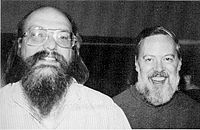
\includegraphics{Ken_n_dennis}
    \caption{肯·汤普逊(左)和丹尼斯·里奇(右)}
    \label{fig:ken}
\end{figure}
Linux~操作系统(Linux),是一类计算机操作系统的统称。Linux~操作系统的内核的名字也是~“Linux”。
Linux~操作系统也是自由软件和开放源代码发展中最著名的例子。严格来讲,Linux~这个词本身只表
示~Linux~内核,但在实际上人们已经习惯了用~Linux~来形容整个基于~Linux~内核,并且使用~GNU~
工程各种工具和数据库的操作系统(也被称为~GNU/Linux~)。基于这些组
件的~Linux~软件被称为~Linux~发行版。

Linux内核最初只是由芬兰人林纳斯·托瓦兹(Linus
Torvalds),见图\ref{fig:linus},在赫尔辛基大学上学时出于
个人爱好而编写的,当时他并不满意~Minix~这个教学用的操作系统,部分因为只能在有限硬件上运行。
最初的设想中,Linux~是一种类似~Minix~这样的一种操作系统。Linux~的第一个版本在1991年9月
被大学~FTP server~管理员~Ari Lemmke~发布在~Internet~上,最初~Torvalds~称这个内核的名称为
~"Freax",意思是自由("free")和奇异("freak")的结合字,并且
附上了~"X"~这个常用的字母,以配合所谓的~Unix-like~的系统。但是~FTP server~管理员
嫌原来的命名~“Freax”~的名称不好听,把内核的称呼改成~“Linux”~,当时仅有10000行代码,仍必须
运行于~Minix~操作系统之上,并且必须使用硬盘开机;随后在10月份第二个版本(0.02版)
就发布了,同时这位芬兰赫尔辛基的大学生在~comp.os.minix~上发布一则消息\par
\begin{center}
\fbox{\parbox[t]{0.8\textwidth}{
Hello everybody out there using minix-\\
I'm doing a (free) operation system (just a hobby,\\
won't be big and professional like gnu) for 386(486) AT clones.}}
\end{center}
\begin{figure}[htbp]
    \centering
    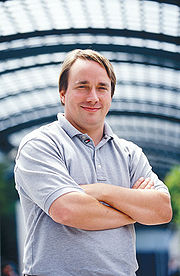
\includegraphics{Linus_Torvalds}
    \caption{Linus Torvalds}
    \label{fig:linus}
\end{figure}

\section{UNIX~历史}
\label{sec:history}
UNIX~的历史开始于1969年~ken Thompson,Dennis Ritchie~(即著名的~K\&G~,~C~语言的发明人)
与一群人在一部~PDP-7~上进行的一些工作,后来这个系统变成了~UNIX。\par
主要大事件:
\begin{itemize}
    \item V1(1971):第一版的UNIX,以~PDP-11/20的汇编语言写成。
        包括文件系统,~fork、roff、ed~等软件。
    \item V4(1973):以~C~语言从头写过,这使得~UNIX~修改容易,可以在几个月内移
        植到新的硬件平台上。最初C语言是为~UNIX~设计的,所以~C~与~UNIX~间有紧密的关系。
    \item V6(1975):第一个在贝尔实验室外(尤其是大学中)广为流传的~UNIX~版本。
        这也是~UNIX~分支的起点与广受欢迎的开始。1.xBSD (PDP-II)就是由这个版本衍生出来的。
    \item V7(1979):在许多UNIX玩家的心目中,这是“最后一个真正的~UNIX,”
        这个版本包括一个完整的~K\&RC~编译器,Bourne
        shell。V7~移植到~VAX~机器后称为~32V。
\end{itemize}
\section{UNIX~家谱}
目前开发~UNIX(System V)的公司是~Unix System Laboratories
(USL)。USL~本为~AT\&T~所有,1993年初被~Novell~收购。Novell~于1993年末将~UNIX~这个注册商标
转让给~X/Open~组织。

\label{sec:family}

详细的~UNIX~编年史\url{http://www.levenez.com/unix/}。

\section{表格样本}
\label{chap1:sample:table}

\subsection{基本表格}
\label{sec:basictable}

模板中关于表格的宏包有三个: \textsf{booktabs}、\textsf{array} 和
\textsf{longtabular},命令有一个 \verb|\hlinewd|。三线表可以用 \textsf{booktabs}
提供的 \verb|\toprule|、\verb|\midrule| 和 \verb|\bottomrule|。它们与
\textsf{longtable} 能很好的配合使用。如果表格比较简单的话可以直接用命令
\verb|hlinewd{xpt}| 控制。
\begin{table}[htb]
  \centering
  \begin{minipage}[t]{0.8\linewidth} % 如果想在表格中使用脚注,minipage是个不错的办法
  \caption[模板文件]{模板文件。如果表格的标题很长,那么在表格索引中就会很不美
    观,所以要像 chapter 那样在前面用中括号写一个简短的标题。这个标题会出现在索
    引中。}
  \label{tab:template-files}
    \begin{tabular*}{\linewidth}{lp{10cm}}
      \toprule[1.5pt]
      {\heiti 文件名} & {\heiti 描述} \\\midrule[1pt]
      tongjithesis.cls & 模板类文件。\footnote{表格中的脚注}\\
      tongjithesis.cfg & 模板配置文件\footnote{再来一个}。\\
      tongjibib.bst    & 参考文献 Bibtex 样式文件。\\
      tongjitils.sty   & 常用的包和命令写在这里,减轻主文件的负担。\\
       shuji.tex & 书脊示例文档\\
 ref/ & 示例文档参考文献目录\\
 data/ & 示例文档章节具体内容\\
 figures/ & 示例文档图片路径\\
 tongjitils.sty & 为示例文档加载其它宏包\\\hline
 \textbf{TongjiThesisReadme.pdf} & 用户手册(本文档)\\
      \bottomrule[1.5pt]
    \end{tabular*}
  \end{minipage}
\end{table}



首先来看一个最简单的表格。表 \ref{tab:template-files} 列举了本模板主要文件及其功
能。请大家注意三线表中各条线对应的命令。这个例子还展示了如何在表格中正确使用脚注。
由于 \LaTeX{} 本身不支持在表格中使用 \verb|\footnote|,所以我们不得不将表格放在
小页中,而且最好将表格的宽度设置为小页的宽度,这样脚注看起来才更美观。

\subsection{表格下方标注数据来源}
\label{sec:tabsource}

我们经常会在表格下方标注数据来源,或者对表格里面的条目进行解释。前面的脚注是一种
不错的方法,如果你不喜欢脚注。那么完全可以在表格后面自己写注释,比如表~\ref{tab:tabexamp1}。
\begin{table}[h]
  \centering
  \caption{复杂表格示例 1}
  \label{tab:tabexamp1}
  \begin{minipage}[t]{0.8\textwidth}
    \begin{tabularx}{\linewidth}{|l|X|X|X|X|}
      \hline
 \multirow{2}*{\backslashbox{x}{y}}  & \multicolumn{2}{c|}{First Half} & \multicolumn{2}{c|}{Second Half}\\\cline{2-5}
      & 1st Qtr &2nd Qtr&3rd Qtr&4th Qtr \\ \hline
      East$^{*}$ &   20.4&   27.4&   90&     20.4 \\
      West$^{**}$ &   30.6 &   38.6 &   34.6 &  31.6 \\ \hline
    \end{tabularx}\\[2pt]
    \footnotesize 注:数据来源《\tongjithesis{} 使用手册》。\\
    *:东部\\
    **:西部
  \end{minipage}
\end{table}

此外,表~\ref{tab:tabexamp1} 同时还演示了另外两个功能:1)通过 \textsf{tabularx} 的
 \texttt{|X|} 扩展实现表格自动放大;2)通过命令 \verb|\backslashbox| 在表头部分
插入反斜线。

为了使我们的例子更接近实际情况,我会在必要的时候插入一些“无关”文字,以免太多图
表同时出现,导致排版效果不太理想。第一个出场的当然是我的最爱:风流潇洒、骏马绝尘、
健笔凌云的{\heiti 李太白}了。

李白,字太白,陇西成纪人。凉武昭王暠九世孙。或曰山东人,或曰蜀人。白少有逸才,志
气宏放,飘然有超世之心。初隐岷山,益州长史苏颋见而异之,曰:“是子天才英特,可比
相如。”天宝初,至长安,往见贺知章。知章见其文,叹曰:“子谪仙人也。”言于明皇,
召见金銮殿,奏颂一篇。帝赐食,亲为调羹,有诏供奉翰林。白犹与酒徒饮于市,帝坐沉香
亭子,意有所感,欲得白为乐章,召入,而白已醉。左右以水颒面,稍解,援笔成文,婉丽
精切。帝爱其才,数宴见。白常侍帝,醉,使高力士脱靴。力士素贵,耻之,摘其诗以激杨
贵妃。帝欲官白,妃辄沮止。白自知不为亲近所容,恳求还山。帝赐金放还。乃浪迹江湖,
终日沉饮。永王璘都督江陵,辟为僚佐。璘谋乱,兵败,白坐长流夜郎,会赦得还。族人阳
冰为当涂令,白往依之。代宗立,以左拾遗召,而白已卒。文宗时,诏以白歌诗、裴旻剑舞、
张旭草书为三绝云。集三十卷。今编诗二十五卷。\hfill\pozhehao《全唐诗》诗人小传

\subsection{浮动体的并排放置}
浮动体的并排放置一般有两种情况:1)二者没有关系,为两个独立的浮动体;2)二者隶属
于同一个浮动体。对表格来说并排表格既可以像表~\ref{tab:parallel1}、表~\ref{tab:parallel2}
使用小页环境,也可以如表~\ref{tab:subtable} 使用子表格来做。图的例子参见第~\ref{sec:multifig} 节。
\begin{table}[h]
\noindent\begin{minipage}{0.5\textwidth}
\centering
\caption{第一个并排子表格}
\label{tab:parallel1}
\begin{tabular}{p{2cm}p{2cm}}
\toprule[1.5pt]
111 & 222 \\\midrule[1pt]
222 & 333 \\\bottomrule[1.5pt]
\end{tabular}
\end{minipage}
\begin{minipage}{0.5\textwidth}
\centering
\caption{第二个并排子表格}
\label{tab:parallel2}
\begin{tabular}{p{2cm}p{2cm}}
\toprule[1.5pt]
111 & 222 \\\midrule[1pt]
222 & 333 \\\bottomrule[1.5pt]
\end{tabular}
\end{minipage}
\end{table}

然后就是忧国忧民,诗家楷模杜工部了。杜甫,字子美,其先襄阳人,曾祖依艺为巩令,因
居巩。甫天宝初应进士,不第。后献《三大礼赋》,明皇奇之,召试文章,授京兆府兵曹参
军。安禄山陷京师,肃宗即位灵武,甫自贼中遁赴行在,拜左拾遗。以论救房琯,出为华州
司功参军。关辅饥乱,寓居同州同谷县,身自负薪采梠,餔糒不给。久之,召补京兆府功曹,
道阻不赴。严武镇成都,奏为参谋、检校工部员外郎,赐绯。武与甫世旧,待遇甚厚。乃于
成都浣花里种竹植树,枕江结庐,纵酒啸歌其中。武卒,甫无所依,乃之东蜀就高適。既至
而適卒。是岁,蜀帅相攻杀,蜀大扰。甫携家避乱荆楚,扁舟下峡,未维舟而江陵亦乱。乃
溯沿湘流,游衡山,寓居耒阳。卒年五十九。元和中,归葬偃师首阳山,元稹志其墓。天宝
间,甫与李白齐名,时称李杜。然元稹之言曰:“李白壮浪纵恣,摆去拘束,诚亦差肩子美
矣。至若铺陈终始,排比声韵,大或千言,次犹数百,词气豪迈,而风调清深,属对律切,
而脱弃凡近,则李尚不能历其藩翰,况堂奥乎。”白居易亦云:“杜诗贯穿古今,  尽工尽
善,殆过于李。”元、白之论如此。盖其出处劳佚,喜乐悲愤,好贤恶恶,一见之于诗。而
又以忠君忧国、伤时念乱为本旨。读其诗可以知其世,故当时谓之“诗史”。旧集诗文共六
十卷,今编诗十九卷。

\begin{table}
\centering
\caption{并排子表格}
\label{tab:subtable}
\subcaptionbox{第一个子表格}
{
  \begin{tabular}{p{2cm}p{2cm}}
  \toprule[1.5pt]
  111 & 222 \\\midrule[1pt]
  222 & 333 \\\bottomrule[1.5pt]
  \end{tabular}
}
\hskip2cm
\subcaptionbox{第二个子表格}
{
  \begin{tabular}{p{2cm}p{2cm}}
  \toprule[1.5pt]
  111 & 222 \\\midrule[1pt]
  222 & 333 \\\bottomrule[1.5pt]
  \end{tabular}
}
\end{table}

\subsection{非常复杂非常漂亮的表格}
不可否认 \LaTeX{} 的表格功能没有想象中的那么强大,不过只要你足够认真,足够细致,那么
同样可以排出来非常复杂非常漂亮的表格。请参看表~\ref{tab:tabexamp2}。
\begin{table}[hb]
  \centering\dawu[1.3]
  \caption{复杂表格示例 2}
  \label{tab:tabexamp2}
  \begin{tabular}[c]{|c|m{0.8in}|c|c|c|c|c|}\hline
    \multicolumn{2}{|c|}{Network Topology} & \# of nodes &
    \multicolumn{3}{c|}{\# of clients} & Server \\\hline
    GT-ITM & Waxman Transit-Stub & 600 &
    \multirow{2}{2em}{2\%}&
    \multirow{2}{2em}{10\%}&
    \multirow{2}{2em}{50\%}&
    \multirow{2}{1.2in}{Max. Connectivity}\\\cline{1-3}
    \multicolumn{2}{|c|}{Inet-2.1} & 6000 & & & &\\\hline
    \multirow{2}{1in}{Xue} & Rui  & Ni &\multicolumn{4}{c|}{\multirow{2}*{\tongjithesis}}\\\cline{2-3}
    & \multicolumn{2}{c|}{ABCDEF} &\multicolumn{4}{c|}{} \\\hline
\end{tabular}
\end{table}

最后就是清新飘逸、文约意赅、空谷绝响的王大侠了。王维,字摩诘,河东人。工书画,与
弟缙俱有俊才。开元九年,进士擢第,调太乐丞。坐累为济州司仓参军,历右拾遗、监察御
史、左补阙、库部郎中,拜吏部郎中。天宝末,为给事中。安禄山陷两都,维为贼所得,服
药阳喑,拘于菩提寺。禄山宴凝碧池,维潜赋诗悲悼,闻于行在。贼平,陷贼官三等定罪,
特原之,责授太子中允,迁中庶子、中书舍人。复拜给事中,转尚书右丞。维以诗名盛于开
元、天宝间,宁薛诸王驸马豪贵之门,无不拂席迎之。得宋之问辋川别墅,山水绝胜,与道
友裴迪,浮舟往来,弹琴赋诗,啸咏终日。笃于奉佛,晚年长斋禅诵。一日,忽索笔作书
数纸,别弟缙及平生亲故,舍笔而卒。赠秘书监。宝应中,代宗问缙:“朕常于诸王坐闻维
乐章,今存几何?”缙集诗六卷,文四卷,表上之。敕答云,卿伯氏位列先朝,名高希代。
抗行周雅,长揖楚辞。诗家者流,时论归美。克成编录,叹息良深。殷璠谓维诗词秀调雅,
意新理惬。在泉成珠,著壁成绘。苏轼亦云:“维诗中有画,画中有诗也。”今编诗四卷。

要想用好论文模板还是得提前学习一些 \TeX/\LaTeX{}的相关知识,具备一些基本能力,掌
握一些常见技巧,否则一旦遇到问题还真是比较麻烦。我们见过很多这样的同学,一直以来
都是使用 Word 等字处理工具,以为 \LaTeX{}模板的用法也应该类似,所以就沿袭同样的思
路来对待这种所见非所得的排版工具,结果被折腾的焦头烂额,疲惫不堪。

\subsection{续表 :表格长度超过一页}
如果您要排版的表格长度超过一页,那么推荐使用 \textsf{longtable} 或者 \textsf{supertabular}
宏包,模板对 \textsf{longtable} 进行了相应的设置,所以用起来可能简单一些。
表~\ref{tab:performance} 就是 \textsf{longtable} 的简单示例。
\begin{longtable}[c]{c*{6}{r}}
\caption{实验数据}\label{tab:performance}\\
\toprule[1.5pt]
 测试程序 & \multicolumn{1}{c}{正常运行} & \multicolumn{1}{c}{同步} & \multicolumn{1}{c}{检查点} & \multicolumn{1}{c}{卷回恢复}
& \multicolumn{1}{c}{进程迁移} & \multicolumn{1}{c}{检查点} \\
& \multicolumn{1}{c}{时间 (s)}& \multicolumn{1}{c}{时间 (s)}&
\multicolumn{1}{c}{时间 (s)}& \multicolumn{1}{c}{时间 (s)}& \multicolumn{1}{c}{
  时间 (s)}&  文件(KB)\\\midrule[1pt]
\endfirsthead
\multicolumn{7}{c}{续表~\thetable\hskip1em 实验数据}\\
\toprule[1.5pt]
 测试程序 & \multicolumn{1}{c}{正常运行} & \multicolumn{1}{c}{同步} & \multicolumn{1}{c}{检查点} & \multicolumn{1}{c}{卷回恢复}
& \multicolumn{1}{c}{进程迁移} & \multicolumn{1}{c}{检查点} \\
& \multicolumn{1}{c}{时间 (s)}& \multicolumn{1}{c}{时间 (s)}&
\multicolumn{1}{c}{时间 (s)}& \multicolumn{1}{c}{时间 (s)}& \multicolumn{1}{c}{
  时间 (s)}&  文件(KB)\\\midrule[1pt]
\endhead
\hline
\multicolumn{7}{r}{续下页}
\endfoot
\endlastfoot
CG.A.2 & 23.05 & 0.002 & 0.116 & 0.035 & 0.589 & 32491 \\
CG.A.4 & 15.06 & 0.003 & 0.067 & 0.021 & 0.351 & 18211 \\
CG.A.8 & 13.38 & 0.004 & 0.072 & 0.023 & 0.210 & 9890 \\
CG.B.2 & 867.45 & 0.002 & 0.864 & 0.232 & 3.256 & 228562 \\
CG.B.4 & 501.61 & 0.003 & 0.438 & 0.136 & 2.075 & 123862 \\
CG.B.8 & 384.65 & 0.004 & 0.457 & 0.108 & 1.235 & 63777 \\
MG.A.2 & 112.27 & 0.002 & 0.846 & 0.237 & 3.930 & 236473 \\
MG.A.4 & 59.84 & 0.003 & 0.442 & 0.128 & 2.070 & 123875 \\
MG.A.8 & 31.38 & 0.003 & 0.476 & 0.114 & 1.041 & 60627 \\
MG.B.2 & 526.28 & 0.002 & 0.821 & 0.238 & 4.176 & 236635 \\
MG.B.4 & 280.11 & 0.003 & 0.432 & 0.130 & 1.706 & 123793 \\
MG.B.8 & 148.29 & 0.003 & 0.442 & 0.116 & 0.893 & 60600 \\
LU.A.2 & 2116.54 & 0.002 & 0.110 & 0.030 & 0.532 & 28754 \\
LU.A.4 & 1102.50 & 0.002 & 0.069 & 0.017 & 0.255 & 14915 \\
LU.A.8 & 574.47 & 0.003 & 0.067 & 0.016 & 0.192 & 8655 \\
LU.B.2 & 9712.87 & 0.002 & 0.357 & 0.104 & 1.734 & 101975 \\
LU.B.4 & 4757.80 & 0.003 & 0.190 & 0.056 & 0.808 & 53522 \\
LU.B.8 & 2444.05 & 0.004 & 0.222 & 0.057 & 0.548 & 30134 \\
EP.A.2 & 123.81 & 0.002 & 0.010 & 0.003 & 0.074 & 1834 \\
EP.A.4 & 61.92 & 0.003 & 0.011 & 0.004 & 0.073 & 1743 \\
EP.A.8 & 31.06 & 0.004 & 0.017 & 0.005 & 0.073 & 1661 \\
EP.B.2 & 495.49 & 0.001 & 0.009 & 0.003 & 0.196 & 2011 \\
EP.B.4 & 247.69 & 0.002 & 0.012 & 0.004 & 0.122 & 1663 \\
EP.B.8 & 126.74 & 0.003 & 0.017 & 0.005 & 0.083 & 1656 \\
CG.A.2 & 23.05 & 0.002 & 0.116 & 0.035 & 0.589 & 32491 \\
CG.A.4 & 15.06 & 0.003 & 0.067 & 0.021 & 0.351 & 18211 \\
CG.A.8 & 13.38 & 0.004 & 0.072 & 0.023 & 0.210 & 9890 \\
CG.B.2 & 867.45 & 0.002 & 0.864 & 0.232 & 3.256 & 228562 \\
CG.B.4 & 501.61 & 0.003 & 0.438 & 0.136 & 2.075 & 123862 \\
CG.B.8 & 384.65 & 0.004 & 0.457 & 0.108 & 1.235 & 63777 \\
MG.A.2 & 112.27 & 0.002 & 0.846 & 0.237 & 3.930 & 236473 \\
MG.A.4 & 59.84 & 0.003 & 0.442 & 0.128 & 2.070 & 123875 \\
MG.A.8 & 31.38 & 0.003 & 0.476 & 0.114 & 1.041 & 60627 \\
MG.B.2 & 526.28 & 0.002 & 0.821 & 0.238 & 4.176 & 236635 \\
MG.B.4 & 280.11 & 0.003 & 0.432 & 0.130 & 1.706 & 123793 \\
MG.B.8 & 148.29 & 0.003 & 0.442 & 0.116 & 0.893 & 60600 \\
LU.A.2 & 2116.54 & 0.002 & 0.110 & 0.030 & 0.532 & 28754 \\
LU.A.4 & 1102.50 & 0.002 & 0.069 & 0.017 & 0.255 & 14915 \\
LU.A.8 & 574.47 & 0.003 & 0.067 & 0.016 & 0.192 & 8655 \\
LU.B.2 & 9712.87 & 0.002 & 0.357 & 0.104 & 1.734 & 101975 \\
LU.B.4 & 4757.80 & 0.003 & 0.190 & 0.056 & 0.808 & 53522 \\
LU.B.8 & 2444.05 & 0.004 & 0.222 & 0.057 & 0.548 & 30134 \\
EP.A.2 & 123.81 & 0.002 & 0.010 & 0.003 & 0.074 & 1834 \\
EP.A.4 & 61.92 & 0.003 & 0.011 & 0.004 & 0.073 & 1743 \\
EP.A.8 & 31.06 & 0.004 & 0.017 & 0.005 & 0.073 & 1661 \\
EP.B.2 & 495.49 & 0.001 & 0.009 & 0.003 & 0.196 & 2011 \\
EP.B.4 & 247.69 & 0.002 & 0.012 & 0.004 & 0.122 & 1663 \\
EP.B.8 & 126.74 & 0.003 & 0.017 & 0.005 & 0.083 & 1656 \\
\bottomrule[1.5pt]
\end{longtable}

表~\ref{tab:data}~为采用\textsf{supertabular}实现长表格功能的示例。
\begin{center} \tablecaption{电容、电感以及电阻元件不确定时系统鲁棒稳定裕度参数 \label{tab:data}}
\tablefirsthead{
\toprule
\multicolumn{1}{c}{T$\left(^{\circ}C\right)$} &
\multicolumn{1}{c}{ $\gamma_C$}  &
\multicolumn{1}{c}{ $\gamma_L$}  &
\multicolumn{1}{c}{ $\gamma_R$} \\}
\tablehead{\multicolumn{4}{c}{\small 续表 \ref{tab:data}~电容、电感以及电阻元件不确定时系统鲁棒稳定裕度参数}\\
\bottomrule
\multicolumn{1}{c}{T$\left(^{\circ}C\right)$} &
\multicolumn{1}{c}{ $\gamma_C$}  &
\multicolumn{1}{c}{ $\gamma_L$}  &
\multicolumn{1}{c}{ $\gamma_R$} \\
\bottomrule}
\tabletail{\bottomrule
\multicolumn{2}{c}{\small 接下页} \\}
\tablelasttail{\bottomrule}
\begin{supertabular}{C{3cm}C{3cm}C{3cm}C{3cm}}
 \midrule
        $-60$                      & $0.8295$              & $0.7854$             & $0.9011$      \\

        $-50$                      & $0.8189$              & $0.7754$             & $0.9011$       \\

        $-40$                      & $0.8096$              & $0.7651$             & $0.9010$      \\

        $-30$                      & $0.7995$              & $0.7547$             & $0.9009$       \\

        $-20$                      & $0.7896$              & $0.7444$             & $0.9009$       \\

        $-10$                      & $0.7800$              & $0.7345$             & $0.9008$       \\

        $0$                         & $0.7707$              & $0.7248$             & $0.9008$        \\

        $10$                      & $0.7617$              & $0.7155$             & $0.9008$         \\

        $20$                      & $0.7529$              & $0.7063$             & $0.9007$       \\

        $30$                      & $0.7442$              & $0.6972$             & $0.9007$       \\

        $40$                      & $0.7356$              & $0.6881$             & $0.9007$      \\

        $50$                      & $0.7269$              & $0.6789$             & $0.9007$       \\

        $60$                      & $0.7182$              & $0.6697$             & $0.9007$       \\

        $70$                      & $0.7095$              & $0.6605$             & $0.9006$       \\

        $80$                      & $0.7009$              & $0.6514$             & $0.9006$       \\

        $90$                      & $0.6925$              & $0.6425$             & $0.9006$      \\

        $100$                    & $0.6846$              & $0.6340$             & $0.9006$       \\

        $110$                    & $0.6774$              & $0.6263$             & $0.9006$      \\

        $120$                    & $0.6711$              & $0.6196$             & $0.9006$      \\

        $130$                    & $0.6659$              & $0.6140$             & $0.9006$       \\

        $140$                    & $0.6621$              & $0.6100$             & $0.9005$       \\

        $150$                    & $0.6599$              & $0.6076$             & $0.9005$       \\

        $160$                    & $0.6594$              & $0.6070$             & $0.9005$       \\

        $170$                    & $0.6606$              & $0.6083$             & $0.9005$       \\

        $180$                    & $0.6634$              & $0.6113$             & $0.9006$       \\

        $190$                    & $0.6676$              & $0.6158$             & $0.9006$       \\

        $200$                    & $0.6729$              & $0.6215$             & $0.9006$       \\

        $210$                    & $0.6789$              & $0.6279$             & $0.9006$       \\

        $220$                    & $0.6848$              & $0.6342$             & $0.9006$       \\

        $230$                    & $0.6902$              & $0.6400$             & $0.9006$      \\

        $240$                    & $0.6945$              & $0.6446$             & $0.9006$       \\

        $250$                    & $0.6978$              & $0.6480$             & $0.9006$       \\

        $260$                    & $0.7006$              & $0.6511$             & $0.9006$       \\

        $270$                    & $0.7050$              & $0.6557$             & $0.9006$      \\

        $280$                    & $0.7148$              & $0.6661$             & $0.9006$      \\
\end{supertabular}
\end{center}

\subsection{设置每列的对齐格式以及宽度}
表~\ref{tab:chap1:IPM_function}使用新定义的\texttt{columntype}设置每列的对齐格式以及宽度。


泉眼无声惜细流,树阴照水爱晴柔。
小荷才露尖尖角,早有蜻蜓立上头。
试问世界上有这么好的诗么?
\begin{verbatim}
门前大桥下
游过一群鸭
快来快来数一数
二四六七八
嘎嘎嘎嘎
真呀真多呀
\end{verbatim}

\begin{table}[h]
\centering
\caption{IPM~智能功率模块引脚功能列表}
\label{tab:chap1:IPM_function}
\begin{tabular}{C{3.6cm}L{1.8cm}L{7.2cm}}
\toprule
\textbf{序号} & \textbf{名称} & \textbf{说明} \\
\midrule
1      & $U_P$   & $U_P$~相控制信号输入端子            \\
2      & $V_{P1}$  & $U_P$~相控制电源端子              \\
3      & $V_{UFB}$ & $U_P$~相驱动电源端子              \\
4      & $V_{UFS}$ & $U_P$~相驱动电源~GND~端子           \\
5      & $V_P$   & $V_P$~相控制信号输入端子            \\
6      & $V_{P1}$  & $V_P$相控制电源端子              \\
7      & $V_{VFB}$ & $V_P$相驱动电源端子              \\
8      & $V_{VFS}$ & $V_P$相驱动电源~GND~端子           \\
9      & $W_P$   & $W_P$~相控制信号输入端子            \\
10     & $V_{P1}$  & $W_P$~相控制电源端子              \\
11     & $V_{PC}$  & $U,V,W$~相控制电源GND端子       \\
12     & $V_{WFB}$ & $W_P$~相驱动电源端子              \\
13     & $V_{WFS}$ & $W_P$~相驱动电源GND端子           \\
14     & $V_{N1}$  & N~侧控制电源端子               \\
15     & $V_{NC}$  & N~侧控制电源~GND~端子            \\
16     & $C_{IN}$  & 短路保护触发电压端子             \\
17     & $C_{FO}$  & $F_O$~输出脉宽设定端子             \\
18     & $F_O$   & $F_O$~输出端子                 \\
19     & $U_N$   & $U_N$~相控制信号输入端子            \\
20     & $V_N$   & $V_N$~相控制信号输入端子            \\
21     & $W_N$   & $W_N$~相控制信号输入端子            \\
22     & $P$    & 逆变器直流输入端子              \\
23     & $U$  & $U$~相输出端子               \\
24     & $V$  & $V$~相输出端子               \\
25     & $W$  & $W$~相输出端子               \\
26     & $N$    & 逆变器直流~GND~ 端子             \\
其余引脚   &      & 虚设端子,不与电路其他端子相连 \\
\bottomrule
\end{tabular}
\end{table}

\subsection{表格内部的换行}
有时候我们希望某个格子是多行的,有很多种方法。
第一种方法,就需要用到 \verb|\tabincell{c}{格子内容}| 命令,如表~\ref{tab:stability_reliability_robust_tab}。
第二种方法,可以用 \verb|p{3cm}| 实现,这样当文字宽度超过指定数值的时候,便会自动换行,且左对齐,但貌似 \verb|\multicolumn|就没法正常显示了,如如表~\ref{tab:stability_reliability_robust_auto}。
大家自行取舍。
或许还有更好的方法,没时间细究了。

\begin{table}[htbp]
\centering
 \caption{稳定性、可靠性、鲁棒性概念的区别}
  \label{tab:stability_reliability_robust_tab}
\begin{tabular}{|C{2cm}|C{2.5cm}|C{2.5cm}|C{3cm}|C{3cm}|}
\hline
                                     &稳定性       &可靠性     &稳定鲁棒性     &性能鲁棒性\\
\hline
 问题产生的原因      &外部扰动  &外部扰动、系统内部参数及结构变化等     &内部模型不确定性与外部摄动  &内部模型不确定性与外部摄动 \\
\hline
          主要关注点       &能抵御外界扰动的幅值和相位的上限  &满足规定参数的工作时间  &在内部模型不确定性和外部摄动情况下,系统能否保持内稳定  &  在内部模型不确定性和外部摄动情况下,系统能否保持动态指标在规定范围内  \\
\hline
            评价指标         &\tabincell{c}{幅值相位裕度、\\Lyapunov渐近\\稳定等}    &\tabincell{c}{可靠度、失效\\率、平均无故\\障时间等 }    & \multicolumn{2}{c|}{\tabincell{c}{ Kharitonov区间理论、H∞控制理论\\、结构奇异值理论(μ理论)等}}     \\
\hline
\end{tabular}
\end{table}


\begin{table}[htbp]
\centering
 \caption{稳定性、可靠性、鲁棒性概念的区别}
  \label{tab:stability_reliability_robust_auto}
\begin{tabular}{|p{2cm}|p{2.5cm}|p{2.5cm}|p{3cm}|p{3cm}|}
\hline
                                     &稳定性       &可靠性     &稳定鲁棒性     &性能鲁棒性\\
\hline
 问题产生的原因      &外部扰动  &外部扰动、系统内部参数及结构变化等     &内部模型不确定性与外部摄动  &内部模型不确定性与外部摄动 \\
\hline
          主要关注点       &能抵御外界扰动的幅值和相位的上限  &满足规定参数的工作时间  &在内部模型不确定性和外部摄动情况下,系统能否保持内稳定  &  在内部模型不确定性和外部摄动情况下,系统能否保持动态指标在规定范围内  \\
\hline
            评价指标         &p幅值相位裕度、Lyapunov渐近稳定等    &可靠度、失效率、平均无故障时间等    &  \multicolumn{2}{c|}{Kharitonov区间理论、H∞控制理论、结构奇异值理论(μ理论)等 咖啡咖啡机}  \\
\hline
\end{tabular}
\end{table}


\subsection{其它}
\label{sec:tableother}
有的同学不想让某个表格或者图片出现在索引里面,那么请使用命令 \verb|\caption*{}|,
这个命令不会给表格编号,也就是出来的只有标题文字而没有“表~XX”,“图~XX”,否则
索引里面序号不连续就显得不伦不类,这也是 \LaTeX{} 里星号命令默认的规则。

有这种需求的多是本科同学的英文资料翻译部分,如果你觉得附录中英文原文中的表格和图
片显示成“  表”和“图”很不协调的话,一个很好的办法就是用 \verb|\caption*|,参数
随便自己写,比如不守规矩的表~1.111 和图~1.111 能满足这种特殊需要(可以参看附录部
分)。
\begin{table}[ht]
\centering
  \begin{minipage}{0.45\linewidth}
  \centering
  \caption*{表~1.111\hskip1em 这是一个手动编号,不出现在索引中的表格。}
  \label{tab:badtabular}
  \begin{picture}(150,50)
    \framebox(150,50)[c]{\tongjithesis}
  \end{picture}
  \end{minipage}\hfill
  \begin{minipage}{0.45\linewidth}
  \centering
  \begin{picture}(150,50)
    \framebox(150,50)[c]{同济人}
  \end{picture}
  \caption*{Figure~1.111\hskip1em 这是一个手动编号,不出现在索引中的图。}
  \label{tab:badfigure}
  \end{minipage}
\end{table}

如果你的确想让它编号,但又不想让它出现在索引中的话,那就自己看看代码改一改吧,我
目前不打算给模板增加这种另类命令。

最后,虽然大家不一定会独立使用小页,但是关于小页中的脚注还是有必要提一下。请看下
面的例子。

\begin{minipage}[t]{\linewidth-2\parindent}
  柳宗元,字子厚(773-819),河东(今永济县)人\footnote{山西永济水饺。},是唐代
  杰出的文学家,哲学家,同时也是一位政治改革家。与韩愈共同倡导唐代古文运动,并称
  韩柳\footnote{唐宋八大家之首二位。}。
\end{minipage}\\[-5pt]

唐朝安史之乱后,宦官专权,藩镇割据,土地兼并日渐严重,社会生产破坏严重,民不聊生。柳宗
元对这种社会现实极为不满,他积极参加了王叔文领导的“永济革新”,并成为这一
运动的中坚人物。他们革除弊政,打击权奸,触犯了宦官和官僚贵族利益,在他们的联合反
扑下,改革失败了,柳宗元被贬为永州司马。

\section{定理环境}
\label{sec:theorem}

给大家演示一下各种和证明有关的环境:

\begin{assumption}
待月西厢下,迎风户半开;隔墙花影动,疑是玉人来。
\begin{eqnarray}
  \label{eq:eqnxmp}
  c & = & a^2 - b^2\\
    & = & (a+b)(a-b)
\end{eqnarray}
\end{assumption}

千辛万苦,历尽艰难,得有今日。然相从数千里,未曾哀戚。今将渡江,方图百年欢笑,如
何反起悲伤?(引自《杜十娘怒沉百宝箱》)

\begin{definition}
子曰:「道千乘之国,敬事而信,节用而爱人,使民以时。」
\end{definition}

千古第一定义!问世间、情为何物,只教生死相许?天南地北双飞客,老翅几回寒暑。欢乐趣,离别苦,就中更有痴儿女。
君应有语,渺万里层云,千山暮雪,只影向谁去?

横汾路,寂寞当年箫鼓,荒烟依旧平楚。招魂楚些何嗟及,山鬼暗谛风雨。天也妒,未信与,莺儿燕子俱黄土。
千秋万古,为留待骚人,狂歌痛饮,来访雁丘处。

\begin{proposition}
 曾子曰:「吾日三省吾身 \pozhehao 为人谋而不忠乎?与朋友交而不信乎?传不习乎?」
\end{proposition}

多么凄美的命题啊!其日牛马嘶,新妇入青庐,奄奄黄昏后,寂寂人定初,我命绝今日,
魂去尸长留,揽裙脱丝履,举身赴清池,府吏闻此事,心知长别离,徘徊庭树下,自挂东南
枝。

\begin{remark}
天不言自高,水不言自流。
\begin{gather*}
\begin{split}
\varphi(x,z)
&=z-\gamma_{10}x-\gamma_{mn}x^mz^n\\
&=z-Mr^{-1}x-Mr^{-(m+n)}x^mz^n
\end{split}\\[6pt]
\begin{align} \zeta^0&=(\xi^0)^2,\\
\zeta^1 &=\xi^0\xi^1,\\
\zeta^2 &=(\xi^1)^2,
\end{align}
\end{gather*}
\end{remark}

天尊地卑,乾坤定矣。卑高以陈,贵贱位矣。 动静有常,刚柔断矣。方以类聚,物以群分,
吉凶生矣。在天成象,在地成形,变化见矣。鼓之以雷霆,润之以风雨,日月运行,一寒一
暑,乾道成男,坤道成女。乾知大始,坤作成物。乾以易知,坤以简能。易则易知,简则易
从。易知则有亲,易从则有功。有亲则可久,有功则可大。可久则贤人之德,可大则贤人之
业。易简,而天下矣之理矣;天下之理得,而成位乎其中矣。

\begin{axiom}
两点间直线段距离最短。
\begin{align}
x&\equiv y+1\pmod{m^2}\\
x&\equiv y+1\mod{m^2}\\
x&\equiv y+1\pod{m^2}
\end{align}
\end{axiom}

《彖曰》:大哉乾元,万物资始,乃统天。云行雨施,品物流形。大明始终,六位时成,时
乘六龙以御天。乾道变化,各正性命,保合大和,乃利贞。首出庶物,万国咸宁。

《象曰》:天行健,君子以自强不息。潜龙勿用,阳在下也。见龙再田,德施普也。终日乾
乾,反复道也。或跃在渊,进无咎也。飞龙在天,大人造也。亢龙有悔,盈不可久也。用九,
天德不可为首也。   

\begin{lemma}
《猫和老鼠》是我最爱看的动画片。
\begin{multline*}%\tag*{[a]} % 这个不出现在索引中
\int_a^b\biggl\{\int_a^b[f(x)^2g(y)^2+f(y)^2g(x)^2]
 -2f(x)g(x)f(y)g(y)\,dx\biggr\}\,dy \\
 =\int_a^b\biggl\{g(y)^2\int_a^bf^2+f(y)^2
  \int_a^b g^2-2f(y)g(y)\int_a^b fg\biggr\}\,dy
\end{multline*}
\end{lemma}

行行重行行,与君生别离。相去万余里,各在天一涯。道路阻且长,会面安可知。胡马依北
风,越鸟巢南枝。相去日已远,衣带日已缓。浮云蔽白日,游子不顾返。思君令人老,岁月
忽已晚。  弃捐勿复道,努力加餐饭。

\begin{theorem}\label{the:theorem1}
犯我强汉者,虽远必诛\hfill \pozhehao 陈汤(汉)
\end{theorem}
\begin{subequations}
\begin{align}
y & = 1 \\
y & = 0
\end{align}
\end{subequations}
道可道,非常道。名可名,非常名。无名天地之始;有名万物之母。故常无,欲以观其妙;
常有,欲以观其徼。此两者,同出而异名,同谓之玄。玄之又玄,众妙之门。上善若水。水
善利万物而不争,处众人之所恶,故几于道。曲则全,枉则直,洼则盈,敝则新,少则多,
多则惑。人法地,地法天,天法道,道法自然。知人者智,自知者明。胜人者有力,自胜
者强。知足者富。强行者有志。不失其所者久。死而不亡者寿。

\begin{proof}
燕赵古称多感慨悲歌之士。董生举进士,连不得志于有司,怀抱利器,郁郁适兹土,吾
知其必有合也。董生勉乎哉?

夫以子之不遇时,苟慕义强仁者,皆爱惜焉,矧燕、赵之士出乎其性者哉!然吾尝闻
风俗与化移易,吾恶知其今不异于古所云邪?聊以吾子之行卜之也。董生勉乎哉?

吾因子有所感矣。为我吊望诸君之墓,而观于其市,复有昔时屠狗者乎?为我谢
曰:“明天子在上,可以出而仕矣!” \hfill\pozhehao 韩愈《送董邵南序》
\end{proof}

\begin{corollary}
  四川话配音的《猫和老鼠》是世界上最好看最好听最有趣的动画片。
\begin{alignat}{3}
V_i & =v_i - q_i v_j, & \qquad X_i & = x_i - q_i x_j,
 & \qquad U_i & = u_i,
 \qquad \text{for $i\ne j$;}\label{eq:B}\\
V_j & = v_j, & \qquad X_j & = x_j,
  & \qquad U_j & u_j + \sum_{i\ne j} q_i u_i.
\end{alignat}
\end{corollary}

迢迢牵牛星,皎皎河汉女。
纤纤擢素手,札札弄机杼。
终日不成章,泣涕零如雨。
河汉清且浅,相去复几许。
盈盈一水间,脉脉不得语。

\begin{example}
  大家来看这个例子。
\begin{equation}
\label{ktc}
\left\{\begin{array}{l}
\nabla f({\mbox{\boldmath $x$}}^*)-\sum\limits_{j=1}^p\lambda_j\nabla g_j({\mbox{\boldmath $x$}}^*)=0\\[0.3cm]
\lambda_jg_j({\mbox{\boldmath $x$}}^*)=0,\quad j=1,2,\cdots,p\\[0.2cm]
\lambda_j\ge 0,\quad j=1,2,\cdots,p.
\end{array}\right.
\end{equation}
\end{example}

\begin{exercise}
  清列出 Andrew S. Tanenbaum 和 W. Richard Stevens 的所有著作。
\end{exercise}

\begin{conjecture} \textit{Poincare Conjecture} If in a closed three-dimensional
  space, any closed curves can shrink to a point continuously, this space can be
  deformed to a sphere.
\end{conjecture}

\begin{problem}
 回答还是不回答,是个问题。
\end{problem}

如何引用定理~\ref{the:theorem1} 呢?加上 \verb|label| 使用 \verb|ref| 即可。妾发
初覆额,折花门前剧。郎骑竹马来,绕床弄青梅。同居长干里,两小无嫌猜。 十四为君妇,
羞颜未尝开。低头向暗壁,千唤不一回。十五始展眉,愿同尘与灰。常存抱柱信,岂上望夫
台。 十六君远行,瞿塘滟滪堆。五月不可触,猿声天上哀。门前迟行迹,一一生绿苔。苔深
不能扫,落叶秋风早。八月蝴蝶来,双飞西园草。感此伤妾心,坐愁红颜老。

\section{参考文献}
\label{sec:bib}
当然参考文献可以直接写 bibitem,虽然费点功夫,但是好控制,各种格式可以自己随意改
写。

本模板推荐使用 biblatex 包,因此工具链为: tex、biber、tex、tex
以下默认使用数字式的引用,这些例子都是为数字式引用准备的,如果你喜欢使用 author year 的引用,可在cls中搜索 biblatex 进行设置。

看看这个例子,关于书的\cite{tex, companion,
ColdSources}, 还有这些\cite{Krasnogor2004e, clzs,
zjsw},关于杂志的\cite{ELIDRISSI94,
  MELLINGER96, SHELL02},硕士论文\cite{zhubajie, metamori2004},博士论文
\cite{shaheshang, FistSystem01},标准文件\cite{IEEE-1363},会议论文\cite{DPMG,kocher99},技术报告\cite{NPB2}。中文参
考文献\cite{cnarticle}。试一下很多个参考文献的情况吧\cite{BogdanSLOPEAdaptiveVariable2014,GossmannIdentificationsignificantgenetic2015,AlbrechtTopologicalapproachfuzzy1999,AlbrechtTopologicalConceptsHierarchies2001,AlbrechtTopologicaltheoryfuzziness1999,MoriasiModelevaluationguidelines2007,Jdatamodels2003}。

有时候不想要上标,那么可以这样 \parencite{shaheshang},这个非常重要。%若使用老版本natbib,则需要使用命令: \inlinecite{}



\section{公式}
\label{sec:equation}
贝叶斯公式如式~(\ref{equ:chap1:bayes}),其中 $p(y|\mathbf{x})$ 为后验;
$p(\mathbf{x})$ 为先验;分母 $p(\mathbf{x})$ 为归一化因子。
\begin{equation}
\label{equ:chap1:bayes}
p(y|\mathbf{x}) = \frac{p(\mathbf{x},y)}{p(\mathbf{x})}=
\frac{p(\mathbf{x}|y)p(y)}{p(\mathbf{x})}
\end{equation}

论文里面公式越多,\TeX{} 就越 happy。再看一个 \textsf{amsmath} 的例子:
\newcommand{\envert}[1]{\left\lvert#1\right\rvert}
\begin{equation}\label{detK2}
\det\mathbf{K}(t=1,t_1,\dots,t_n)=\sum_{I\in\mathbf{n}}(-1)^{\envert{I}}
\prod_{i\in I}t_i\prod_{j\in I}(D_j+\lambda_jt_j)\det\mathbf{A}
^{(\lambda)}(\overline{I}|\overline{I})=0.
\end{equation}

前面定理示例部分列举了很多公式环境,可以说把常见的情况都覆盖了,大家在写公式的时
候一定要好好看 \textsf{amsmath} 的文档,并参考模板中的用法:
\begin{multline*}%\tag{[b]} % 这个出现在索引中的
\int_a^b\biggl\{\int_a^b[f(x)^2g(y)^2+f(y)^2g(x)^2]
 -2f(x)g(x)f(y)g(y)\,dx\biggr\}\,dy \\
 =\int_a^b\biggl\{g(y)^2\int_a^bf^2+f(y)^2
  \int_a^b g^2-2f(y)g(y)\int_a^b fg\biggr\}\,dy
\end{multline*}

其实还可以看看这个多级规划:
\begin{equation}\label{bilevel}
\left\{\begin{array}{l}
\max\limits_{{\mbox{\footnotesize\boldmath $x$}}} F(x,y_1^*,y_2^*,\cdots,y_m^*)\\[0.2cm]
\mbox{subject to:}\\[0.1cm]
\qquad G(x)\le 0\\[0.1cm]
\qquad(y_1^*,y_2^*,\cdots,y_m^*)\mbox{ solves problems }(i=1,2,\cdots,m)\\[0.1cm]
\qquad\left\{\begin{array}{l}
    \max\limits_{{\mbox{\footnotesize\boldmath $y_i$}}}f_i(x,y_1,y_2,\cdots,y_m)\\[0.2cm]
    \mbox{subject to:}\\[0.1cm]
    \qquad g_i(x,y_1,y_2,\cdots,y_m)\le 0.
    \end{array}\right.
\end{array}\right.
\end{equation}
这些跟规划相关的公式都来自于刘宝碇老师《不确定规划》的课件。

对于复杂公式,采用\verb|\frac|方式书写公式不美观,如~\ref{equ5}所示。 

\begin{equation}
\label{equ5}
  S_s\left(s\right)  =\frac{1}{1+\frac{\left(1+sR_2C_1\right)\cdot\left[1+s\left(R_1+R_3\right)C_3\right]}{\left[{sR_1}\cdot\left(C_1+C_2\right)\cdot\left[1+s\frac{R_2C_1C_2}{C_1+C_2}\right]\cdot\left(1+sR_3C_3\right)\cdot{V_m}\right]}\cdot\frac{V_{out}}{D}\cdot\frac{1}{s^2LC+{s}\frac{L}{R_L}+1}\cdot\frac{R_y}{R_x+R_y}}
\end{equation}

为了使得多级分式中二级以上分子分母大小与普通分式大小相同,定义新的命令\verb|\FS|,具体定义见~.cls文件。采用\verb|\FS|命令书写多级公式
效果如下

\begin{small}
\begin{equation}
\label{equ6}
  S_s\left(s\right) =\FS{1}{1+\FS{\left(1+sR_2C_1\right)\cdot\left[1+s\left(R_1+R_3\right)C_3\right]}{\left[{sR_1}\cdot\left(C_1+C_2\right)\cdot\left[1+s\FS{R_2C_1C_2}{C_1+C_2}\right]\cdot\left(1+sR_3C_3\right)\cdot{V_m}\right]}\cdot\FS{V_{out}}{D}\cdot\FS{1}{s^2LC+{s}\FS{L}{R_L}+1}\cdot\FS{R_y}{R_x+R_y}}
\end{equation}
\end{small}
\section{破折号}
\label{sec:pozhehao}

中文破折号为一个两个字宽垂直居中的直线,输入法直接得到的破折号是两个断开的小短线
(——),这看起来不舒服。所以我定义了一个破折号的命令 \verb|\pozhehao|,请看几个
例子:
\begin{itemize}
\item 这是一个 \pozhehao 破折号
  \begin{enumerate}[(1)]
  \item 同时也可以看看
  \item 不同列表环境的间距
  \end{enumerate}
\item 看起来这个要好一些
\item 破折号 \pozhehao 就说到这里。
\end{itemize}

默认的列表环境上下间距很大,模板将其重定义为 \textsf{paralist} 中的压缩环境,看起
来要好一些。如果还是不满意,自己也可以调 \verb|\itemsep| 的。\textsf{paralist} 还
可以方便的指定标签的样式。



\chapter{中华人民共和国}
\label{cha:china}

\section{图的例子}
\label{sec:other}

在第~\ref{cha:intro} 章中我们学习了贝叶斯公式~(\ref{equ:chap1:bayes}),这里我们复
习一下:
\begin{equation}
\label{equ:chap2:bayes}
p(y|\mathbf{x}) = \frac{p(\mathbf{x},y)}{p(\mathbf{x})}=
\frac{p(\mathbf{x}|y)p(y)}{p(\mathbf{x})}
\end{equation}

\subsection{绘图}
\label{sec:draw}

本模板不再预先装载任何绘图包(如 \textsf{pstricks,pgf} 等),完全由你自己来决定。
个人觉得 \textsf{pgf} 不错,不依赖于 Postscript。此外还有很多针对 \LaTeX{} 的
 GUI 作图工具,如 XFig(jFig), WinFig, Tpx, Ipe, Dia, Inkscape, LaTeXPiX,
jPicEdt, jaxdraw 等等。

\subsection{插图}
\label{sec:graphs}
关于子图形的使用细节请参看 \textsf{subcaption} 的说明文档。

\subsection{一个图形}
\label{sec:onefig}
一般图形都是处在浮动环境中。之所以称为浮动是指最终排版效果图形的位置不一定与源文
件中的位置对应\footnote{This is not a bug, but a feature of
\LaTeX!},这也是刚使 用 \LaTeX{}
同学可能遇到的问题。如果要强制固定浮动图形的位置,请使用
\textsf{float} 宏包, 它提供了 \texttt{[H]}
参数,比如图~\ref{fig:heythere}。
\begin{figure}[H] % use float package if you want it here
  \centering
  
\includegraphics[height=2cm]{hello.jpg}
  \caption{插个图插个图}
  \label{fig:heythere}
\end{figure}

大学之道,在明明德,在亲民,在止于至善。知止而后有定;定而后能静;静而后能安;安
而后能虑;虑而后能得。物有本末,事有终始。知所先后,则近道矣。古之欲明明德于天
下者,先治其国;欲治其国者,先齐其家;欲齐其家者,先修其身;欲修其身者,先正其心;
欲正其心者,先诚其意;欲诚其意者,先致其知;致知在格物。物格而后知至;知至而后
意诚;意诚而后心正;心正而后身 修;身修而后家齐;家齐而后国治;国治而后天下
平。自天子以至于庶人,壹是皆以修身为本。其本乱而未治者 否矣。其所厚者薄,而其所
薄者厚,未之有也!

\hfill \pozhehao《大学》


\subsection{简单子图}
\label{sec:multifig}

如果多个图形相互独立,并不共用一个图形计数器,那么用 \verb|minipage| 或者
\verb|parbox| 就可以。否则,请参看图~\ref{fig:big1},它包含两个小图,分别是图~\ref{fig:subfig1}
和图~\ref{fig:subfig2}。推荐使用 \verb|\subcaption|,不要再用\verb|\subfloat|,\verb|\subfigure| 和 \verb|\subtable|了。
\begin{figure} %[h]
  \centering%
  \subcaptionbox{第一个小图形\label{fig:subfig1}}{%    
    
\includegraphics[height=2cm]{tongji-fig-logo.png}}\hspace{4em}%
  \subcaptionbox{第二个小图形。如果标题很长的话,它会自动换行,这个 caption 就是这样的例子\label{fig:subfig2}}{%    
    
\includegraphics[height=2cm]{tongji-text-logo.png}}
  \caption{包含子图形的大图形}
  \label{fig:big1}
\end{figure}

古之学者必有师。师者,所以传道受业解惑也。人非生而知之者,孰能无惑?惑而不从师,
其为惑也,终不解矣。生乎吾前,其闻道也固先乎吾,吾从而师之;生乎吾後,其闻道也亦
先乎吾,吾从而师之。吾师道也,夫庸知其年之先後生於吾乎!是故无贵无贱无长无少,道
之所存,师之所存也。

嗟乎!师道之不传也久矣,欲人之无惑也难矣。古之圣人,其出人也远矣,犹且从师而问焉;
今之众人,其下圣人也亦远矣,而耻学於师。是故圣益圣,愚益愚。圣人之所以为圣,愚
人之所以为愚,其皆出於此乎?爱其子,择师而教之,於其身也,则耻师焉,惑焉。彼童子
之师,授之书而习其句读者,非吾所谓传其道、解其惑者也。句读之不知,惑之不解,或师
焉,或不焉,小学而大遗,吾未见其明也。巫医、乐师、百工之人不耻相师,  士大夫之族
曰“师”曰“弟子”之云者,则群聚而笑之。问之,则曰:彼与彼年相若也,道相似也,位
卑则足羞,官盛则近谀。呜呼!师道之不复,可知矣。巫医、乐师、百工之人。吾子不齿,
今其智乃反不能及,其可怪也欤!圣人无常师。孔子师郯子、苌子、师襄、老聃。郯子之徒,
其贤不及孔子。孔子曰:“三人行,必有我师。”是故弟子不必不如师,师不必贤於弟子。
闻道有先後,术业有专攻,如是而已。

\subsection{复杂子图要注意遮挡}
使用子图的方法如图~\ref{fig:chap2:zitu}所示,使用\texttt{subcaptionbox}环境设置每一个子图,注意\texttt{subcaptionbox}其后需要有括号,以及子图换行时需要使用\texttt{vskip},以免下一排子图会对上一排子图的图名造成遮挡。
\begin{figure}[htbp]
\centering
  \subcaptionbox{第一个小图形}{\label{fig:chap1:zitu:a}
  
\includegraphics[width=5cm]{tongji-fig-logo}\hskip2cm}
  \subcaptionbox{第二个小图形}{\label{fig:chap1:zitu:b}
  
\includegraphics[width=5cm]{tongji-fig-logo}}
\vskip0.5cm
  \subcaptionbox{第三个小图形}{\label{fig:chap1:zitu:c}
  
\includegraphics[width=5cm]{tongji-fig-logo}\hskip2cm}
  \subcaptionbox{第四个小图形}{\label{fig:chap1:zitu:d}
  
\includegraphics[width=5cm]{tongji-fig-logo}}
\caption{多子图用\texttt{subcaptionbox}}\label{fig:chap2:zitu}
\end{figure}


\subsection{多个图形独立}
如果要把编号的两个图形并排,那么小页就非常有用了,如图~\ref{fig:parallel2}:
\begin{figure}
\begin{minipage}{0.48\textwidth}
  \centering
  
\includegraphics[height=2cm]{tongji-whole-logo.png}
  \caption{并排第一个图}
  \label{fig:parallel1}
\end{minipage}\hfill
\begin{minipage}{0.48\textwidth}
  \centering
  
\includegraphics[height=2cm]{tongji-whole-logo.png}
  \caption{并排第二个图}
  \label{fig:parallel2}
\end{minipage}
\end{figure}


李氏子蟠,年十七,好古文、六艺,经传皆通习之,不拘於时,学於余。余嘉其能行古
道,作师说以贻之。

\hfill \pozhehao 韩愈(唐)


\subsection{插图大原则}
同志们,如果遇到问题一定要会搜索,要么看别人的问答,要么看宏包的文档,希望你不要成为重度伸手党。
一点微小的工作,谢谢大家。

\section{插入pdf格式图片的问题}
\label{sec:problem}
在\LaTeX{}中插入高清图片一般有两种方式:1)插入~eps~矢量图,2)插入~pdf~格式图片。在模板测试过程中遇到一个插入
~pdf~格式图片的问题。

问题描述

插入~pdf~格式的图,有时采用~XeLaTeX~编译后,插图被翻转~90~度。有时却不会出现该问题。问题图片如图~\ref{rotatedBode}~所示。
\begin{figure}[H] 
  \centering
  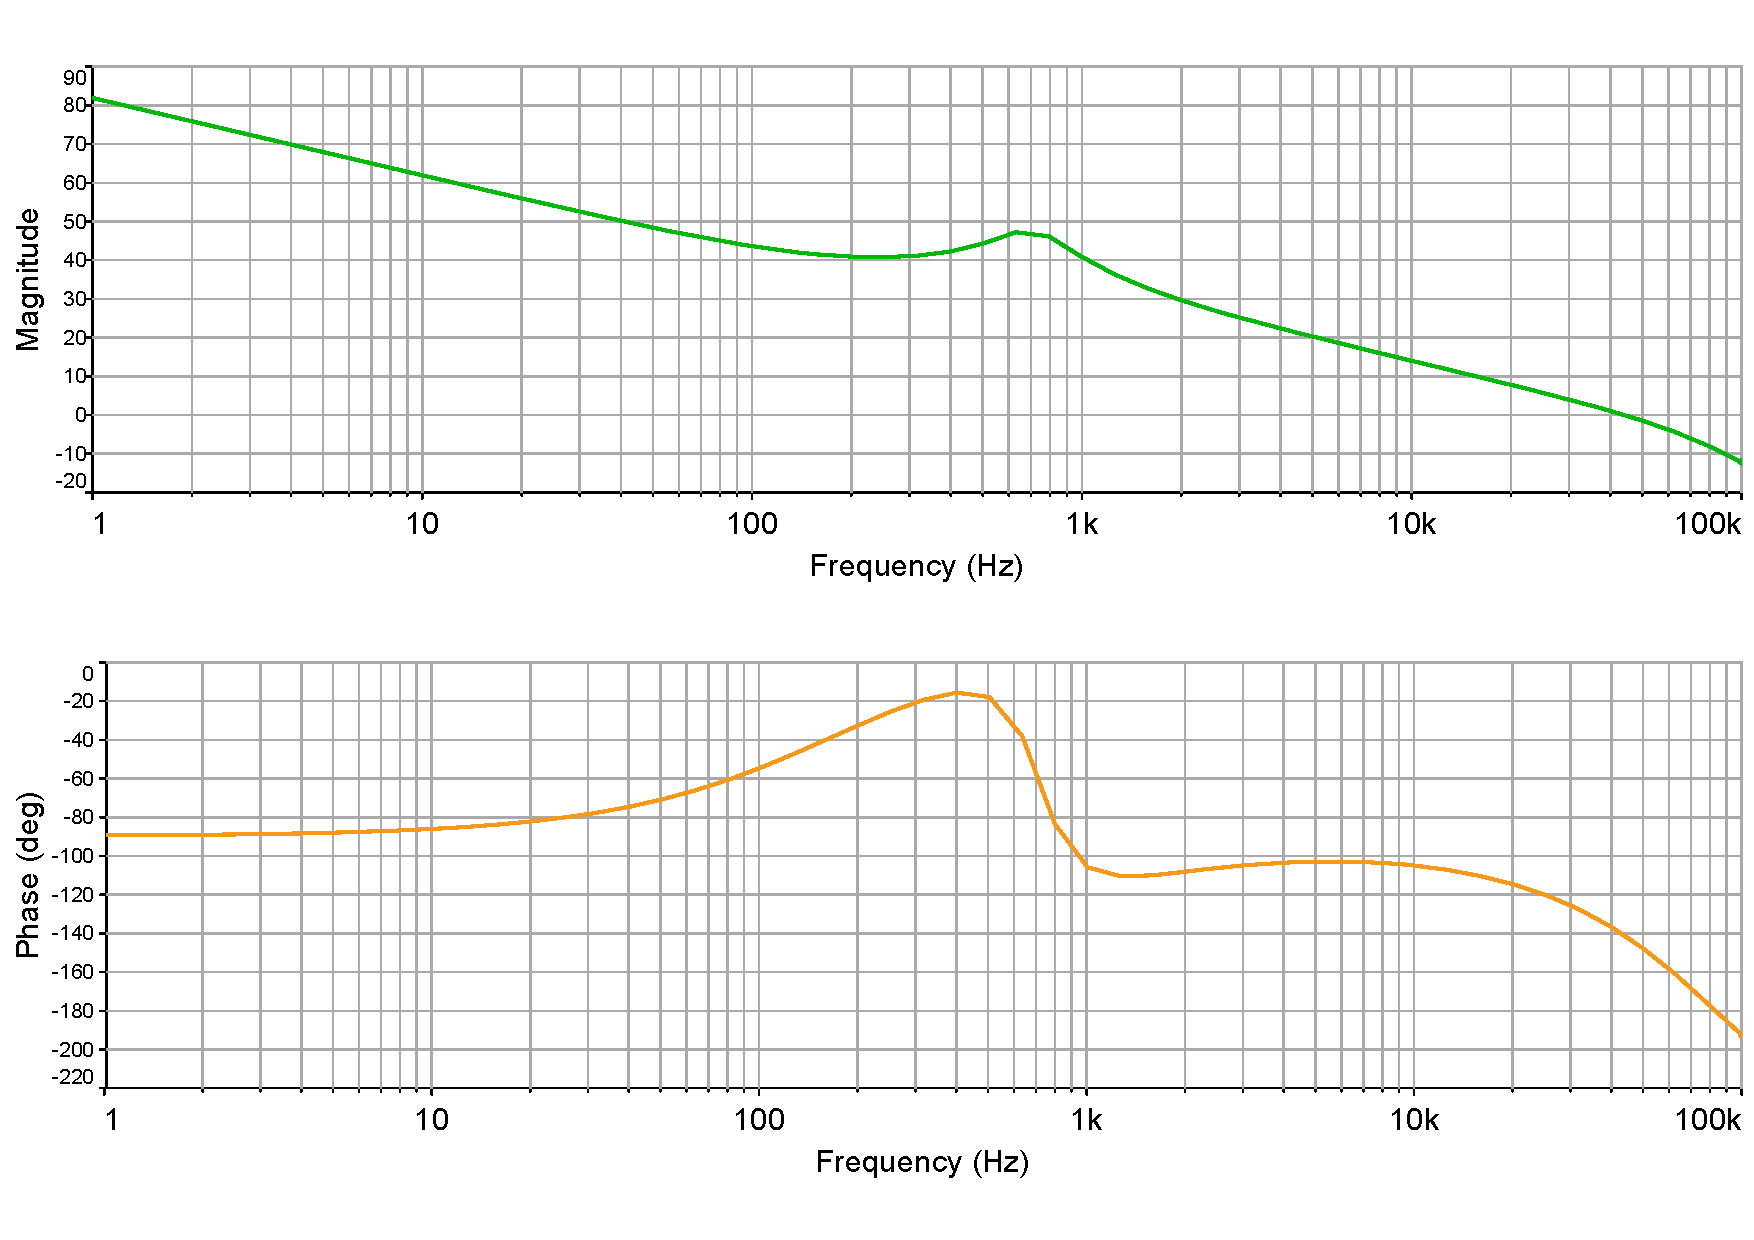
\includegraphics[width=12cm]{BodeGraph.pdf}
  \caption{被自动翻转的bode图}
  \label{rotatedBode}
\end{figure}

问题原因

同一幅图片,XeLaTeX~编译出现图片翻转,而~pdfLaTeX~编译,输出正常。
原因可能是出现在~XeLaTeX~编译过程中会将有些~pdf~文件自身多余的旋转命令编译出来。

问题解决方法

第一种方法(抄自刘海洋大牛的方案):
使用命令\\ \texttt{pdfcrop foo.pdf foo-new.pdf},当然,新文件名可以和旧文件名相同。 这个方法的好处就是 pdfcrop 是texlive自带的,我装的是texlive2017,因此自带了。

第二种方法:采用GhostScript软件消除多余的旋转命令。
\begin{enumerate}
    \item 下载安装~GhostScript~软件,官网为\url{https://www.ghostscript.com/download/gsdnld.html/}
        
    \item 将安装后的bin文件夹地址加入用户环境变量,在我电脑上为~\verb|D:|\verb|\Program Files|\verb|\gs|\verb|\gs9.22|\verb|\bin|
	
    \item cmd~命令行进入想转换图片所在文件夹,执行命令\\gswin32c -sDEVICE=pdfwrite -o newname.pdf  previousname.pdf
              得到一个去除多余旋转命令的~newname.pdf~文件。

    \item 在\LaTeX{}中插入该~pdf~文件,XeLaTeX~编译。
\end{enumerate}

处理之后的图片如图~\ref{Bode}~所示。
\begin{figure}[H] 
  \centering
  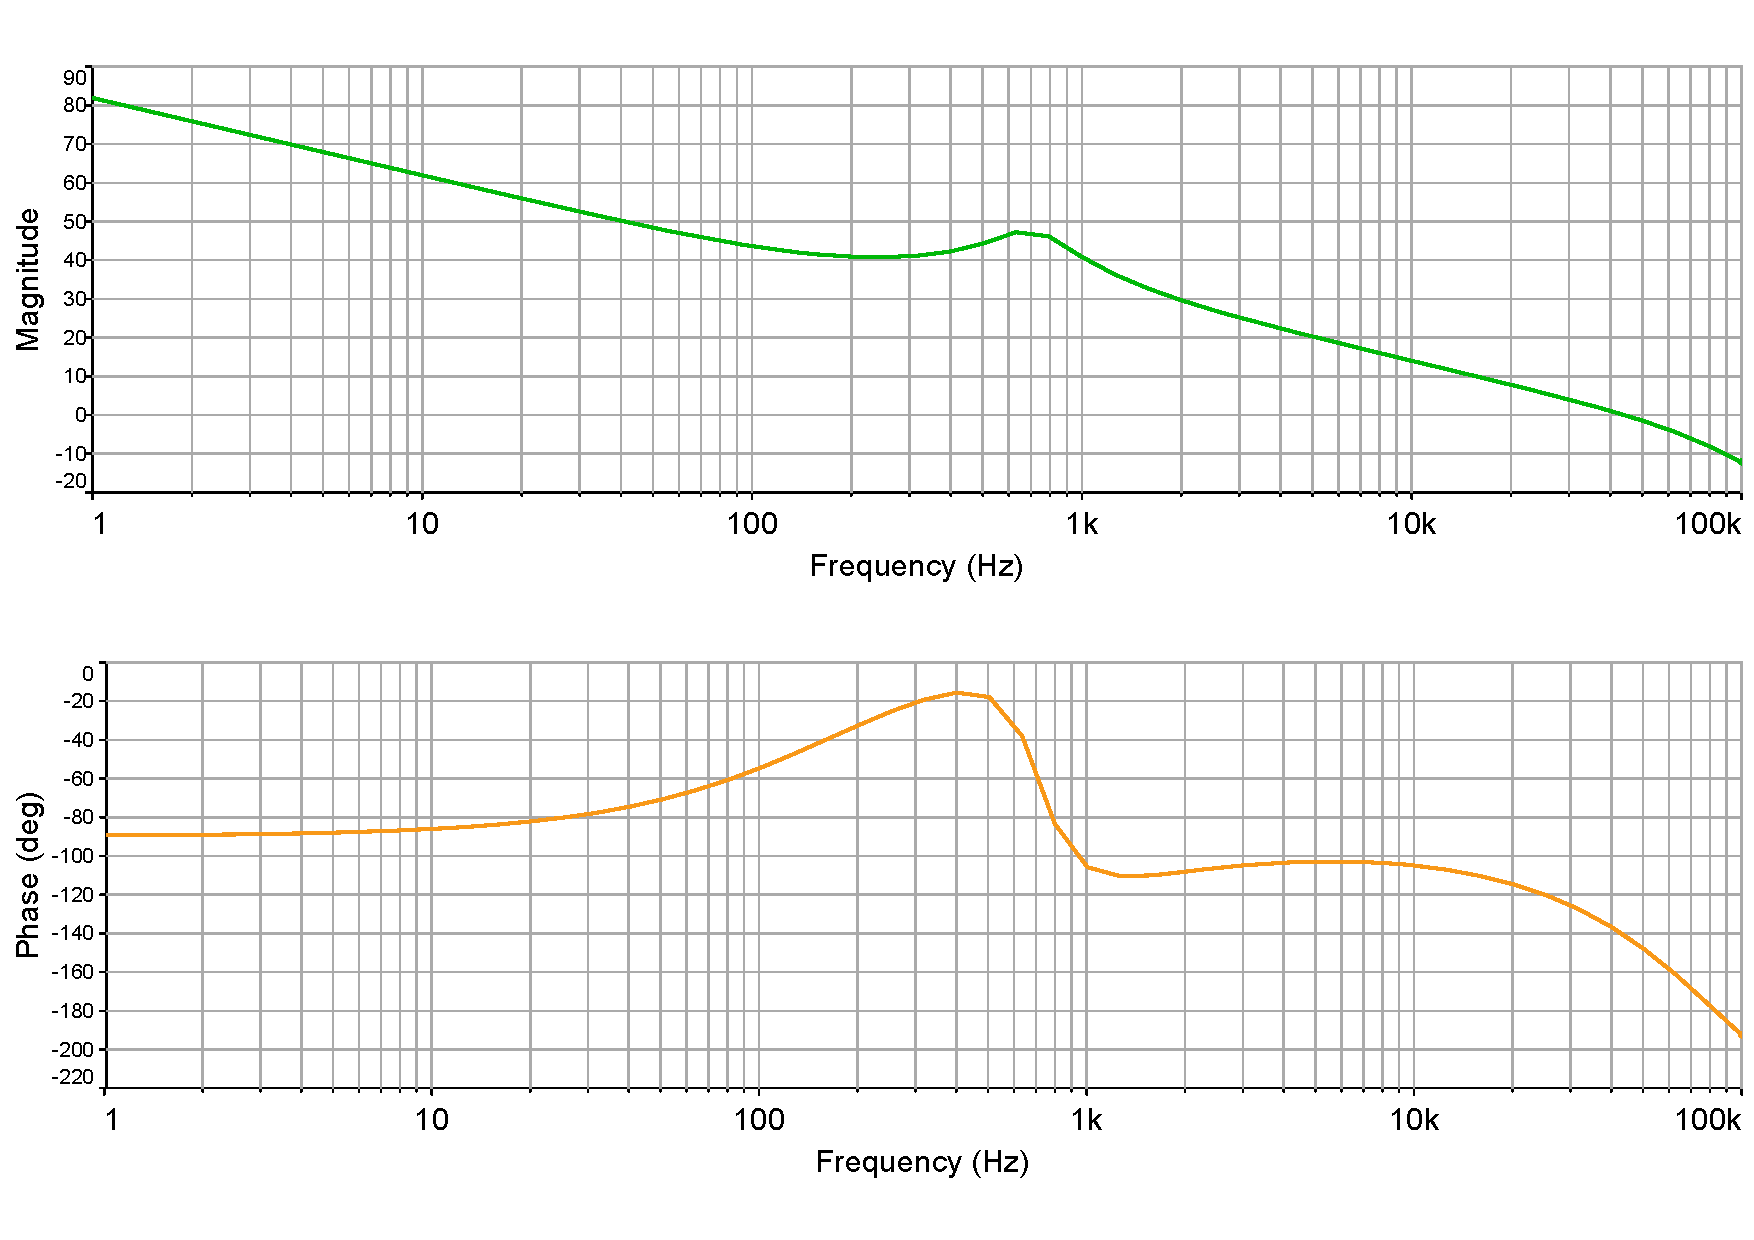
\includegraphics[width=12cm]{Bode.pdf}
  \caption{处理后的bode图}
  \label{Bode}
\end{figure}







%%% 其它部分
\backmatter

% 致谢
\begin{acknowledgement}
衷心感谢导师 xxx 教授和物理系 xxx 副教授对本人的精心指导。他们的言传身教将使
我终生受益。

在美国麻省理工学院化学系进行九个月的合作研究期间,承蒙 xxx 教授热心指导与帮助,不
胜感激。感谢 xx 实验室主任 xx 教授,以及实验室全体老师和同学们的热情帮助和支
持!本课题承蒙国家自然科学基金资助,特此致谢。

感谢 \tongjithesis{},它的存在让我的论文写作轻松自在了许多,让我的论文格式规整漂亮了
许多。
\end{acknowledgement}

% 参考文献
\printTJbibliography


% 附录
\begin{appendix}
\chapter{外文资料原文}
\label{cha:engorg}
As one of the most widely used techniques in operations research, {\em
  mathematical programming} is defined as a means of maximizing a quantity known
as {\em objective function}, subject to a set of constraints represented by
equations and inequalities. Some known subtopics of mathematical programming are
linear programming, nonlinear programming, multiobjective programming, goal
programming, dynamic programming, and multilevel programming$^{[1]}$.

It is impossible to cover in a single chapter every concept of mathematical
programming. This chapter introduces only the basic concepts and techniques of
mathematical programming such that readers gain an understanding of them
throughout the book$^{[2,3]}$.


\section{Single-Objective Programming}
The general form of single-objective programming (SOP) is written
as follows,
\begin{equation}\tag*{(123)} % 如果附录中的公式不想让它出现在公式索引中,那就请
                             % 用 \tag*{xxxx}
\left\{\begin{array}{l}
\max \,\,f(x)\\[0.1 cm]
\mbox{subject to:} \\ [0.1 cm]
\qquad g_j(x)\le 0,\quad j=1,2,\cdots,p
\end{array}\right.
\end{equation}
which maximizes a real-valued function $f$ of
$x=(x_1,x_2,\cdots,x_n)$ subject to a set of constraints.

\newtheorem{mpdef}{Definition}[chapter]
\begin{mpdef}
In SOP, we call $x$ a decision vector, and
$x_1,x_2,\cdots,x_n$ decision variables. The function
$f$ is called the objective function. The set
\begin{equation}\tag*{(456)} % 这里同理,其它不再一一指定。
S=\left\{x\in\Re^n\bigm|g_j(x)\le 0,\,j=1,2,\cdots,p\right\}
\end{equation}
is called the feasible set. An element $x$ in $S$ is called a
feasible solution.
\end{mpdef}

\newtheorem{mpdefop}[mpdef]{Definition}
\begin{mpdefop}
A feasible solution $x^*$ is called the optimal
solution of SOP if and only if
\begin{equation}
f(x^*)\ge f(x)
\end{equation}
for any feasible solution $x$.
\end{mpdefop}

One of the outstanding contributions to mathematical programming was known as
the Kuhn-Tucker conditions\ref{eq:ktc}. In order to introduce them, let us give
some definitions. An inequality constraint $g_j(x)\le 0$ is said to be active at
a point $x^*$ if $g_j(x^*)=0$. A point $x^*$ satisfying $g_j(x^*)\le 0$ is said
to be regular if the gradient vectors $\nabla g_j(x)$ of all active constraints
are linearly independent.

Let $x^*$ be a regular point of the constraints of SOP and assume that all the
functions $f(x)$ and $g_j(x),j=1,2,\cdots,p$ are differentiable. If $x^*$ is a
local optimal solution, then there exist Lagrange multipliers
$\lambda_j,j=1,2,\cdots,p$ such that the following Kuhn-Tucker conditions hold,
\begin{equation}
\label{eq:ktc}
\left\{\begin{array}{l}
    \nabla f(x^*)-\sum\limits_{j=1}^p\lambda_j\nabla g_j(x^*)=0\\[0.3cm]
    \lambda_jg_j(x^*)=0,\quad j=1,2,\cdots,p\\[0.2cm]
    \lambda_j\ge 0,\quad j=1,2,\cdots,p.
\end{array}\right.
\end{equation}
If all the functions $f(x)$ and $g_j(x),j=1,2,\cdots,p$ are convex and
differentiable, and the point $x^*$ satisfies the Kuhn-Tucker conditions
(\ref{eq:ktc}), then it has been proved that the point $x^*$ is a global optimal
solution of SOP.

\subsection{Linear Programming}
\label{sec:lp}

If the functions $f(x),g_j(x),j=1,2,\cdots,p$ are all linear, then SOP is called
a {\em linear programming}.

The feasible set of linear is always convex. A point $x$ is called an extreme
point of convex set $S$ if $x\in S$ and $x$ cannot be expressed as a convex
combination of two points in $S$. It has been shown that the optimal solution to
linear programming corresponds to an extreme point of its feasible set provided
that the feasible set $S$ is bounded. This fact is the basis of the {\em simplex
  algorithm} which was developed by Dantzig as a very efficient method for
solving linear programming.
\begin{table}[ht]
\centering
  \centering
  \caption*{Table~1\hskip1em This is an example for manually numbered table, which
    would not appear in the list of tables}
  \label{tab:badtabular2}
  \begin{tabular}[c]{|c|m{0.8in}|c|c|c|c|c|}\hline
    \multicolumn{2}{|c|}{Network Topology} & \# of nodes &
    \multicolumn{3}{c|}{\# of clients} & Server \\\hline
    GT-ITM & Waxman Transit-Stub & 600 &
    \multirow{2}{2em}{2\%}&
    \multirow{2}{2em}{10\%}&
    \multirow{2}{2em}{50\%}&
    \multirow{2}{1.2in}{Max. Connectivity}\\\cline{1-3}
    \multicolumn{2}{|c|}{Inet-2.1} & 6000 & & & &\\\hline
    \multirow{2}{1in}{Xue} & Rui  & Ni &\multicolumn{4}{c|}{\multirow{2}*{\tongjithesis}}\\\cline{2-3}
    & \multicolumn{2}{c|}{ABCDEF} &\multicolumn{4}{c|}{} \\\hline
\end{tabular}
\end{table}

Roughly speaking, the simplex algorithm examines only the extreme points of the
feasible set, rather than all feasible points. At first, the simplex algorithm
selects an extreme point as the initial point. The successive extreme point is
selected so as to improve the objective function value. The procedure is
repeated until no improvement in objective function value can be made. The last
extreme point is the optimal solution.

\subsection{Nonlinear Programming}

If at least one of the functions $f(x),g_j(x),j=1,2,\cdots,p$ is nonlinear, then
SOP is called a {\em nonlinear programming}.

A large number of classical optimization methods have been developed to treat
special-structural nonlinear programming based on the mathematical theory
concerned with analyzing the structure of problems.
\begin{figure}[h]
  \centering
  
\includegraphics[clip]{tongji-lib-logo.jpg}
  \caption*{Figure~1\hskip1em This is an example for manually numbered figure,
    which would not appear in the list of figures}
  \label{tab:badfigure2}
\end{figure}

Now we consider a nonlinear programming which is confronted solely with
maximizing a real-valued function with domain $\Re^n$.  Whether derivatives are
available or not, the usual strategy is first to select a point in $\Re^n$ which
is thought to be the most likely place where the maximum exists. If there is no
information available on which to base such a selection, a point is chosen at
random. From this first point an attempt is made to construct a sequence of
points, each of which yields an improved objective function value over its
predecessor. The next point to be added to the sequence is chosen by analyzing
the behavior of the function at the previous points. This construction continues
until some termination criterion is met. Methods based upon this strategy are
called {\em ascent methods}, which can be classified as {\em direct methods},
{\em gradient methods}, and {\em Hessian methods} according to the information
about the behavior of objective function $f$. Direct methods require only that
the function can be evaluated at each point. Gradient methods require the
evaluation of first derivatives of $f$. Hessian methods require the evaluation
of second derivatives. In fact, there is no superior method for all
problems. The efficiency of a method is very much dependent upon the objective
function.

\subsection{Integer Programming}

{\em Integer programming} is a special mathematical programming in which all of
the variables are assumed to be only integer values. When there are not only
integer variables but also conventional continuous variables, we call it {\em
  mixed integer programming}. If all the variables are assumed either 0 or 1,
then the problem is termed a {\em zero-one programming}. Although integer
programming can be solved by an {\em exhaustive enumeration} theoretically, it
is impractical to solve realistically sized integer programming problems. The
most successful algorithm so far found to solve integer programming is called
the {\em branch-and-bound enumeration} developed by Balas (1965) and Dakin
(1965). The other technique to integer programming is the {\em cutting plane
  method} developed by Gomory (1959).

\hfill\textit{Uncertain Programming\/}\quad(\textsl{BaoDing Liu, 2006.2})

\section*{References}
\noindent{\itshape NOTE: these references are only for demonstration, they are
  not real citations in the original text.}

\begin{enumerate}[{$[$}1{$]$}]
\item Donald E. Knuth. The \TeX book. Addison-Wesley, 1984. ISBN: 0-201-13448-9
\item Paul W. Abrahams, Karl Berry and Kathryn A. Hargreaves. \TeX\ for the
  Impatient. Addison-Wesley, 1990. ISBN: 0-201-51375-7
\item David Salomon. The advanced \TeX book.  New York : Springer, 1995. ISBN:0-387-94556-3
\end{enumerate}

\chapter{外文资料的调研阅读报告或书面翻译}
\section{单目标规划}
北冥有鱼,其名为鲲。鲲之大,不知其几千里也。化而为鸟,其名为鹏。鹏之背,不知其几
千里也。怒而飞,其翼若垂天之云。是鸟也,海运则将徙于南冥。南冥者,天池也。
\begin{equation}\tag*{(123)}
 p(y|\mathbf{x}) = \frac{p(\mathbf{x},y)}{p(\mathbf{x})}=
\frac{p(\mathbf{x}|y)p(y)}{p(\mathbf{x})}
\end{equation}

吾生也有涯,而知也无涯。以有涯随无涯,殆已!已而为知者,殆而已矣!为善无近名,为
恶无近刑,缘督以为经,可以保身,可以全生,可以养亲,可以尽年。

\subsection{线性规划}
庖丁为文惠君解牛,手之所触,肩之所倚,足之所履,膝之所倚,砉然响然,奏刀騞然,莫
不中音,合于桑林之舞,乃中经首之会。
\begin{table}[ht]
\centering
  \centering
  \caption*{表~1\hskip1em 这是手动编号但不出现在索引中的一个表格例子}
  \label{tab:badtabular3}
  \begin{tabular}[c]{|c|m{0.8in}|c|c|c|c|c|}\hline
    \multicolumn{2}{|c|}{Network Topology} & \# of nodes &
    \multicolumn{3}{c|}{\# of clients} & Server \\\hline
    GT-ITM & Waxman Transit-Stub & 600 &
    \multirow{2}{2em}{2\%}&
    \multirow{2}{2em}{10\%}&
    \multirow{2}{2em}{50\%}&
    \multirow{2}{1.2in}{Max. Connectivity}\\\cline{1-3}
    \multicolumn{2}{|c|}{Inet-2.1} & 6000 & & & &\\\hline
    \multirow{2}{1in}{Xue} & Rui  & Ni &\multicolumn{4}{c|}{\multirow{2}*{\tongjithesis}}\\\cline{2-3}
    & \multicolumn{2}{c|}{ABCDEF} &\multicolumn{4}{c|}{} \\\hline
\end{tabular}
\end{table}

文惠君曰:“嘻,善哉!技盖至此乎?”庖丁释刀对曰:“臣之所好者道也,进乎技矣。始臣之
解牛之时,所见无非全牛者;三年之后,未尝见全牛也;方今之时,臣以神遇而不以目视,
官知止而神欲行。依乎天理,批大郤,导大窾,因其固然。技经肯綮之未尝,而况大坬乎!
良庖岁更刀,割也;族庖月更刀,折也;今臣之刀十九年矣,所解数千牛矣,而刀刃若新发
于硎。彼节者有间而刀刃者无厚,以无厚入有间,恢恢乎其于游刃必有余地矣。是以十九年
而刀刃若新发于硎。虽然,每至于族,吾见其难为,怵然为戒,视为止,行为迟,动刀甚微,
謋然已解,如土委地。提刀而立,为之而四顾,为之踌躇满志,善刀而藏之。”

文惠君曰:“善哉!吾闻庖丁之言,得养生焉。”


\subsection{非线性规划}
孔子与柳下季为友,柳下季之弟名曰盗跖。盗跖从卒九千人,横行天下,侵暴诸侯。穴室枢
户,驱人牛马,取人妇女。贪得忘亲,不顾父母兄弟,不祭先祖。所过之邑,大国守城,小
国入保,万民苦之。孔子谓柳下季曰:“夫为人父者,必能诏其子;为人兄者,必能教其弟。
若父不能诏其子,兄不能教其弟,则无贵父子兄弟之亲矣。今先生,世之才士也,弟为盗
跖,为天下害,而弗能教也,丘窃为先生羞之。丘请为先生往说之。”
\begin{figure}[h]
  \centering
  
\includegraphics{hello}
  \caption*{图~1\hskip1em 这是手动编号但不出现索引中的图片的例子}
  \label{tab:badfigure3}
\end{figure}

柳下季曰:“先生言为人父者必能诏其子,为人兄者必能教其弟,若子不听父之诏,弟不受
兄之教,虽今先生之辩,将奈之何哉?且跖之为人也,心如涌泉,意如飘风,强足以距敌,
辩足以饰非。顺其心则喜,逆其心则怒,易辱人以言。先生必无往。”

孔子不听,颜回为驭,子贡为右,往见盗跖。

\subsection{整数规划}
盗跖乃方休卒徒大山之阳,脍人肝而餔之。孔子下车而前,见谒者曰:“鲁人孔丘,闻将军
高义,敬再拜谒者。”谒者入通。盗跖闻之大怒,目如明星,发上指冠,曰:“此夫鲁国之
巧伪人孔丘非邪?为我告之:尔作言造语,妄称文、武,冠枝木之冠,带死牛之胁,多辞缪
说,不耕而食,不织而衣,摇唇鼓舌,擅生是非,以迷天下之主,使天下学士不反其本,妄
作孝弟,而侥幸于封侯富贵者也。子之罪大极重,疾走归!不然,我将以子肝益昼餔之膳。”


\chapter{其它附录}
其它附录的内容可以放到这里,当然如果你愿意,可以把这部分也放到独立的文件中,然后
将其\verb|\input| 到主文件中。
\end{appendix}

% 个人简历
\begin{resume}
\resumeitem{个人简历:}
\noindent xxxx 年 xx 月 xx 日出生于 xx 省 xx 县。\\
\noindent xxxx 年 9 月考入 xx 大学 xx 系 xx 专业,xxxx 年 7 月本科毕业并获得 xx 学士学位。\\
\noindent xxxx 年 9 月免试进入 xx 大学 xx 系攻读 xx 学位至今。

\resumeitem{发表论文:} % 发表的和录用的合在一起
\begin{enumerate}[{[}1{]}]
\item Yang Y, Ren T L, Zhang L T, et al. Miniature microphone with silicon-
  based ferroelectric thin films. Integrated Ferroelectrics, 2003,
  52:229-235. (SCI 收录, 检索号:758FZ.)
\item 杨轶, 张宁欣, 任天令, 等. 硅基铁电微声学器件中薄膜残余应力的研究. 中国机
  械工程, 2005, 16(14):1289-1291. (EI 收录, 检索号:0534931 2907.)
\item 杨轶, 张宁欣, 任天令, 等. 集成铁电器件中的关键工艺研究. 仪器仪表学报,
  2003, 24(S4):192-193. (EI 源刊.)
\item Yang Y, Ren T L, Zhu Y P, et al. PMUTs for handwriting recognition. In
  press. (已被 Integrated Ferroelectrics 录用. SCI 源刊.)
\item Wu X M, Yang Y, Cai J, et al. Measurements of ferroelectric MEMS
  microphones. Integrated Ferroelectrics, 2005, 69:417-429. (SCI 收录, 检索号
  :896KM.)
\item 贾泽, 杨轶, 陈兢, 等. 用于压电和电容微麦克风的体硅腐蚀相关研究. 压电与声
  光, 2006, 28(1):117-119. (EI 收录, 检索号:06129773469.)
\item 伍晓明, 杨轶, 张宁欣, 等. 基于MEMS技术的集成铁电硅微麦克风. 中国集成电路, 
  2003, 53:59-61.
\end{enumerate}

\resumeitem{研究成果:} % 有就写,没有就删除
\begin{enumerate}[{[}1{]}]
\item 任天令, 杨轶, 朱一平, 等. 硅基铁电微声学传感器畴极化区域控制和电极连接的
  方法: 中国, CN1602118A. (中国专利公开号.)
\item Ren T L, Yang Y, Zhu Y P, et al. Piezoelectric micro acoustic sensor
  based on ferroelectric materials: USA, No.11/215, 102. (美国发明专利申请号.)
\end{enumerate}

\end{resume}

\end{document}
